%% LyX 2.3.5.2 created this file.  For more info, see http://www.lyx.org/.
%% Do not edit unless you really know what you are doing.
\documentclass[english]{scrartcl}
\usepackage[T1]{fontenc}
\usepackage[latin9]{inputenc}
\usepackage{amsmath}
\usepackage{graphicx}
\usepackage[authoryear]{natbib}

\makeatletter
%%%%%%%%%%%%%%%%%%%%%%%%%%%%%% User specified LaTeX commands.
\usepackage{lipsum}
\usepackage{url}
%\usepackage{endfloat}

\usepackage{hyperref}

\newcommand{\QQQ}{\fbox{???}}
\newcommand{\E}{\mathrm{E}\,}
\newcommand{\var}{\mathrm{Var}\,}


\newcommand{\Epost}{\mathrm{E}_\mathrm{post}\,}

\makeatother

\usepackage{babel}
\begin{document}
\title{Bayesian Analysis of the Election Results}
\subtitle{MATH6480, Final Project}
\author{Aleksei Luchinsky}
\maketitle
\begin{abstract}
This is my project
\end{abstract}
\tableofcontents{}

\section{Introduction}

\section{State-Level Analysis}

\subsection{Dataset Description}

I will start my project with the analysis of the United States presidential
election results on the state level. It is well known that there are
52 states in our country and every 4 years people of these states
vote for the person who will be the president of the country during
next presidential term. The voting system in US is little bit complicated,
so simple majority of votes does not guarantee the the person who
got it will be the winner, only electoral college results are important.
In the following, however, we will neglect this step and consider
only numbers of votes, given for each of the candidates.

You can easily find the results of the previous US presidential elections
in the internet. For example, on reference \citet{MIT} number of
votes to each major party are presented in each state for from 2000,
2004, 2008, 2012, 2016, and 2020 years.

It turns out also, that traditionally the candidates represent one
of the major parties and usually people from Democratic or Republican
parties receive noticable number of voted. Results of such parties
as Green, Libertarian, etc, are much smaller. For this reason in the
following I will concentrate only on votes for Democratic and Republican
parties and neglect all others.

In figures \ref{fig:Results-of-2000} and \ref{fig:Results-of-2004}
you can see the election results during 2000 and 2004 years. It is
clear that political interests of different state are different and
some states usually vote for democratic candidates, while the other
are typically republicans. There are also states that are eager to
change their position from year ti year (so called swing states).
For this reason it could be interesting to perform the statistical
analysis of available data at different years.

\begin{figure}
\begin{centering}
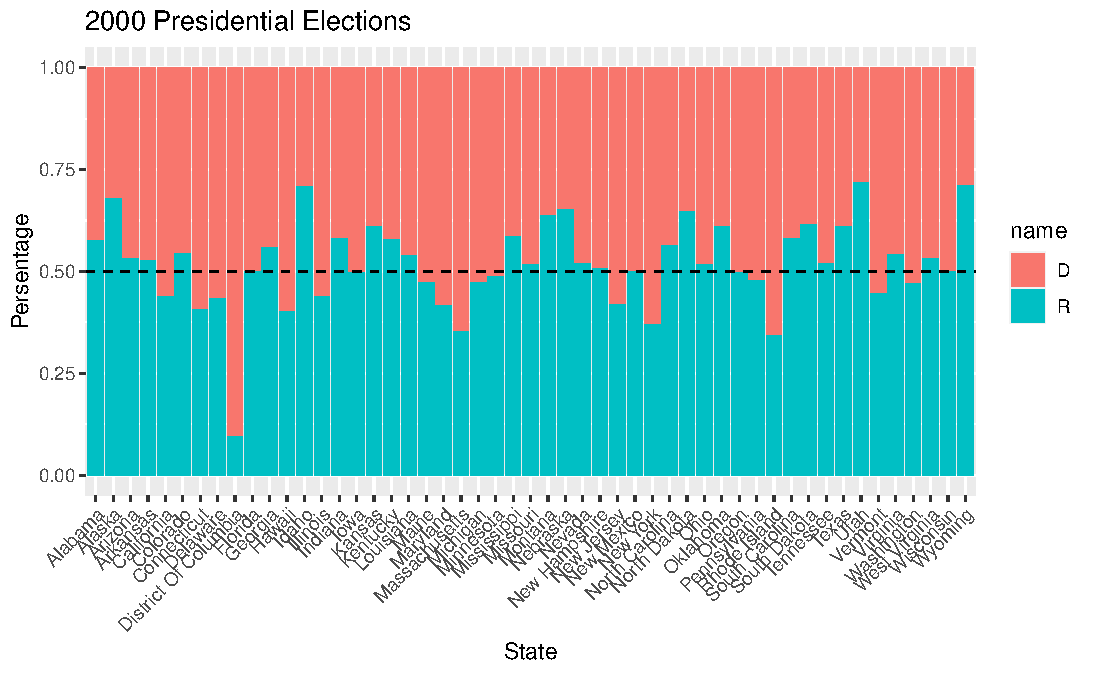
\includegraphics[width=0.9\textwidth]{figs/states_2000_barplot}
\par\end{centering}
\caption{Results of 2000 presidential elections by state\label{fig:Results-of-2000}}
\end{figure}

\begin{figure}
\begin{centering}
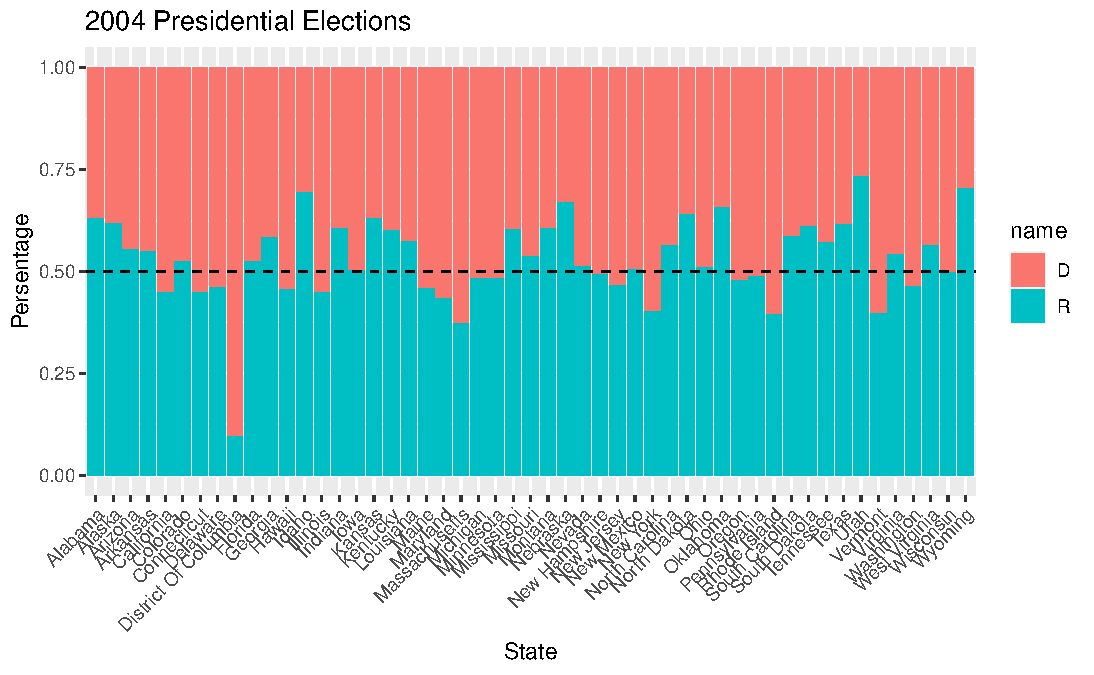
\includegraphics[width=0.9\textwidth]{figs/states_2004_barplot}
\par\end{centering}
\caption{Results of 2004 presidential elections by state\label{fig:Results-of-2004}}
\end{figure}


\subsection{Binomial Model}

\subsubsection{Description}

As it was already mentioned, in our analysis we will neglect results
of small parties and consider only candidates from democratic and
republican parties. In mentioned above data set you can find number
of votes for each year and each sate, in the following I will denote
these numbers as $D_{j}$ and $R_{j}$ respectively\footnote{Note that these numbers are in thousands.}.
Here index $j$ denotes the state under analysis and I neglect the
year index for a while.

In the framework of Bayesian analysis we should start with determine
the form of prior distribution. Since we are talking with selection
of several people for total fixed number, it seems reasonable to use
the binomial distribution in this case:
\begin{align}
D_{j}|\theta_{j}\sim & \text{binom}\left(\theta_{j},V_{j}\right),\label{eq:state-binim-sampling}
\end{align}
where $V_{j}=D_{j}+R_{j}$ is total number of voters and parameters
$\theta_{j}$ represent the percentage of people who prefer democratic
president for each state. It is clear that sampling pdf is equal to
\begin{align*}
p\left(D|\theta\right) & \sim\prod_{j}\theta_{j}^{D_{j}}\left(1-\theta_{j}\right)^{V_{j}-D_{j}},
\end{align*}
where we denote complete vectors $\left\{ D_{1},D_{2},\dots\right\} $
and $\left\{ \theta_{1},\theta_{2},\dots\right\} $ by $D$ and $\theta$
respectively.

As we know, in Baesian theory parameters $\theta$ are by considered
as random numbers by itself and before taking observed data into account
they follow some prior distribution. In principle, one can take any
distribution as a prior, but it is more convenient to take one from
conjugate family to the sampling distribution. As we know, conjugate
distribution for binomial is beta-distribution, so in our analysis
we will use
\begin{align*}
\theta_{j}|a,b\sim & \text{beta}\left(a,b\right)
\end{align*}
with the prior probability density function
\begin{align*}
p\left(\theta|a,b\right)\sim & \prod_{j}\theta_{j}^{a-1}\left(1-\theta_{j}\right)^{b-1}.
\end{align*}
In these expressions $a$ and $b$ are hyper-parameters and we will
discuss their choice later.

The posterior distribution for $\theta_{j}$ can easily derived from
above relations:
\begin{align*}
p\left(\theta_{j}|D_{j},a,b\right)\sim & p\left(D|\theta\right)p(\theta|a,b)\sim\\
 & \prod_{j}\theta_{j}^{a+D_{j}-1}\left(1-\theta_{j}\right)^{b+V_{j}-D_{j}-1},
\end{align*}
which is obviously 
\begin{align}
\theta_{j}\sim & \text{beta}\left(a+D_{j},b+V_{j}-D_{j}\right).\label{eq:state-binom-post}
\end{align}
As you can see, information about election results simply modifies
slightly the values of the distribution parameters without change
of its form (this is the reason for choosing the conjugate beta distribution
as prior).

In order to perform the further analysis we need to select proper
values of hyper-parameters $a$ and $b$. As it was shown in the course,
the marginal posterior distribution for them is
\begin{align}
p\left(a,b|D\right)\sim & p\left(a,b\right)\prod_{j}\frac{\Gamma\left(a+b\right)}{\Gamma\left(a\right)\Gamma\left(b\right)}\frac{\Gamma\left(a+D_{j}\right)\Gamma\left(b+V_{j}-D_{j}\right)}{\Gamma\left(a+b+V_{j}\right)}.\label{eq:state-binom-hyperpost}
\end{align}
This distribution, unfortunately, is not standard, so we should use
some numerical method for simulation.

Thus, the simulation procedure looks as follows:
\begin{enumerate}
\item Draw hyper-parameters $a$, $b$ from some hyper-prior;
\item Use the accept/reject method to select pairs $\left(a,b\right)$ that
follows marginal posterior distribution (\ref{eq:state-binom-hyperpost});
\item For each of the selected pairs $\left(a_{s},b_{s}\right)$ use sampling
distribution (\ref{eq:state-binom-post}) to draw parameters $\theta_{j}$;
\item Use sampling distribution (\ref{eq:state-binim-sampling}) to draw
number of democratic votes $D_{j}$.
\end{enumerate}

\subsubsection{Results}

Let me consider analysis results for year 2004 first.

In figure \ref{fig:states-binom-hyperscatter} you can see the scatter
plot of the hyper-parameters $a$, $b$. s you can see, they are concentrated
near $a\approx10$, $b\approx12$, which gives us an estimate for
mean value of the parameter $\theta$:
\begin{align*}
\E\theta= & \frac{a}{a+b}\approx0.45.
\end{align*}
More detailed calculations (see also histograms in figure \ref{fig:state-binom-mean-var})
show that this mean lies in the range
\begin{align*}
\theta\in & \left[0.43;0.51\right].
\end{align*}

\begin{figure}
\begin{centering}
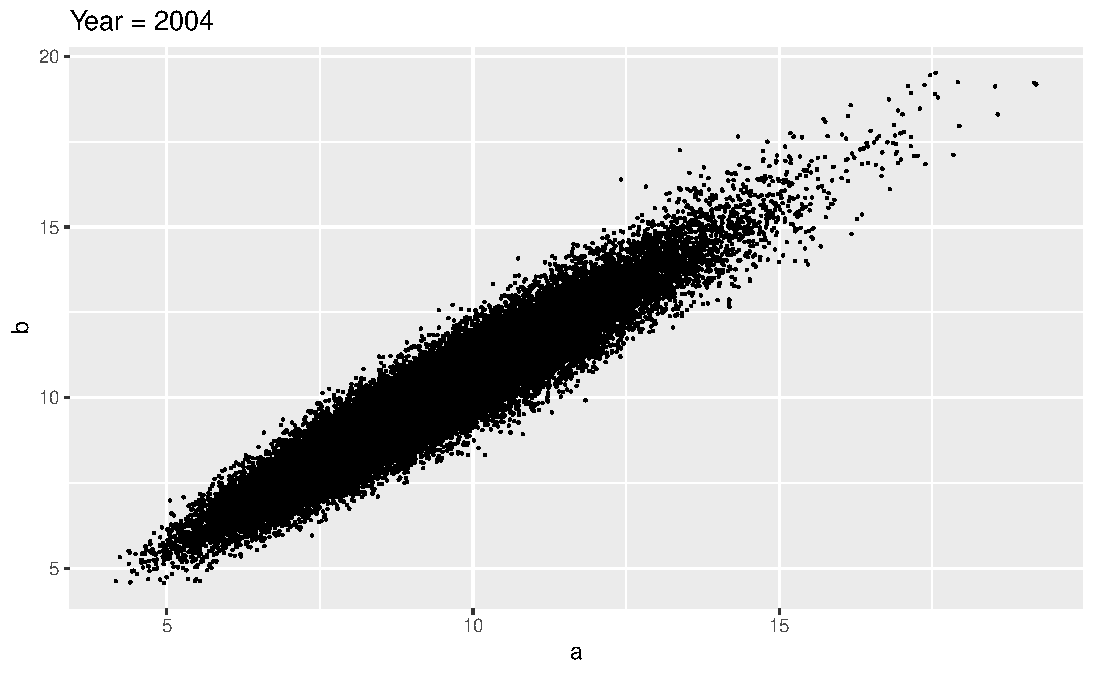
\includegraphics[width=0.9\textwidth]{figs/states_2004_hyper_scatter}
\par\end{centering}
\caption{Scatter Plot of hyper-parameters\label{fig:states-binom-hyperscatter}}

\end{figure}

\begin{figure}
\begin{centering}
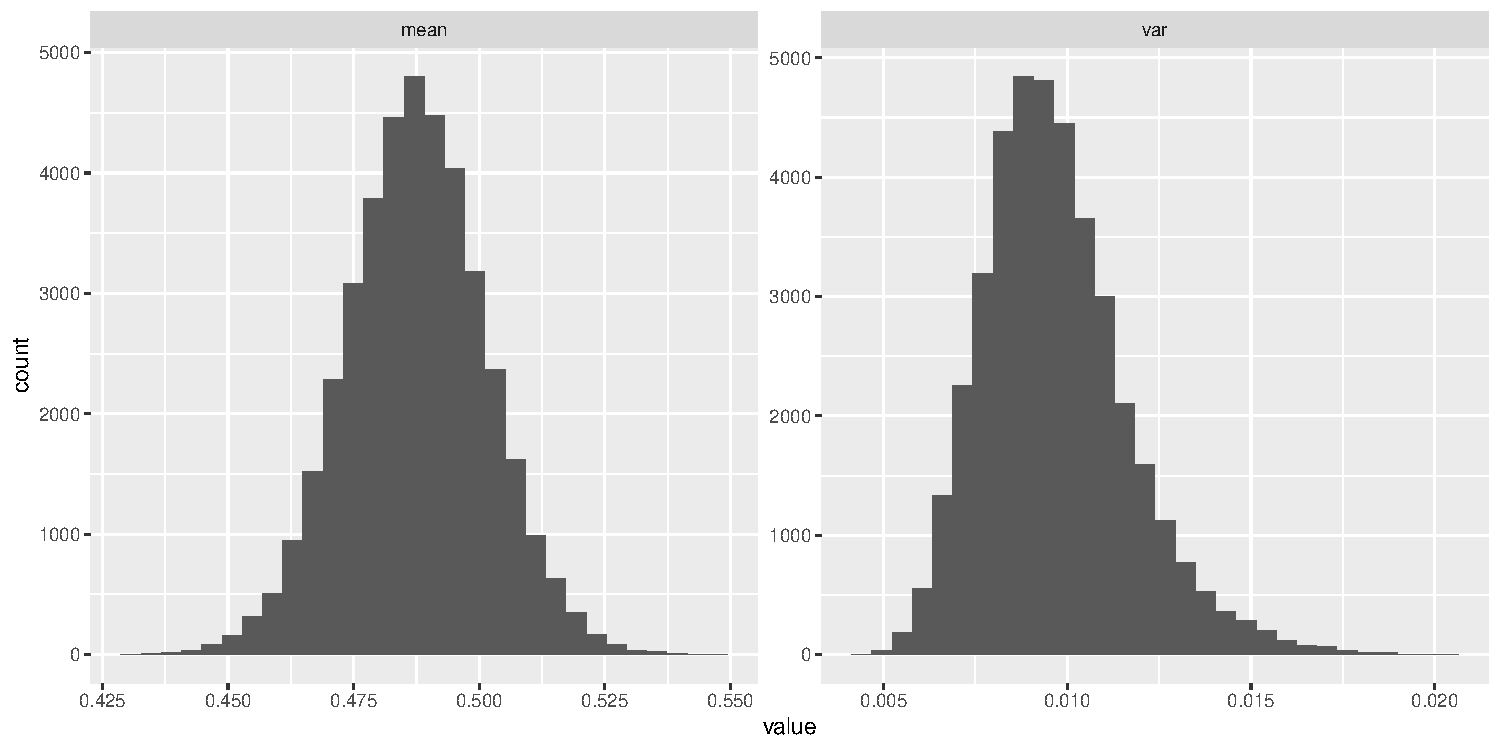
\includegraphics[width=0.9\textwidth]{figs/state_2004_th_mean_var}
\par\end{centering}
\caption{Histograms of $\theta$ mean and variance\label{fig:state-binom-mean-var}}

\end{figure}

Let us now consider predictions for specific states. In figure \ref{fig:state-binom-mean-var}
you can see comparison of the simulation results for Alabama, Florida,
and Alaska with observed in 2004 year values. As you can see, the
agreement is very nice.

\begin{figure}
\begin{centering}
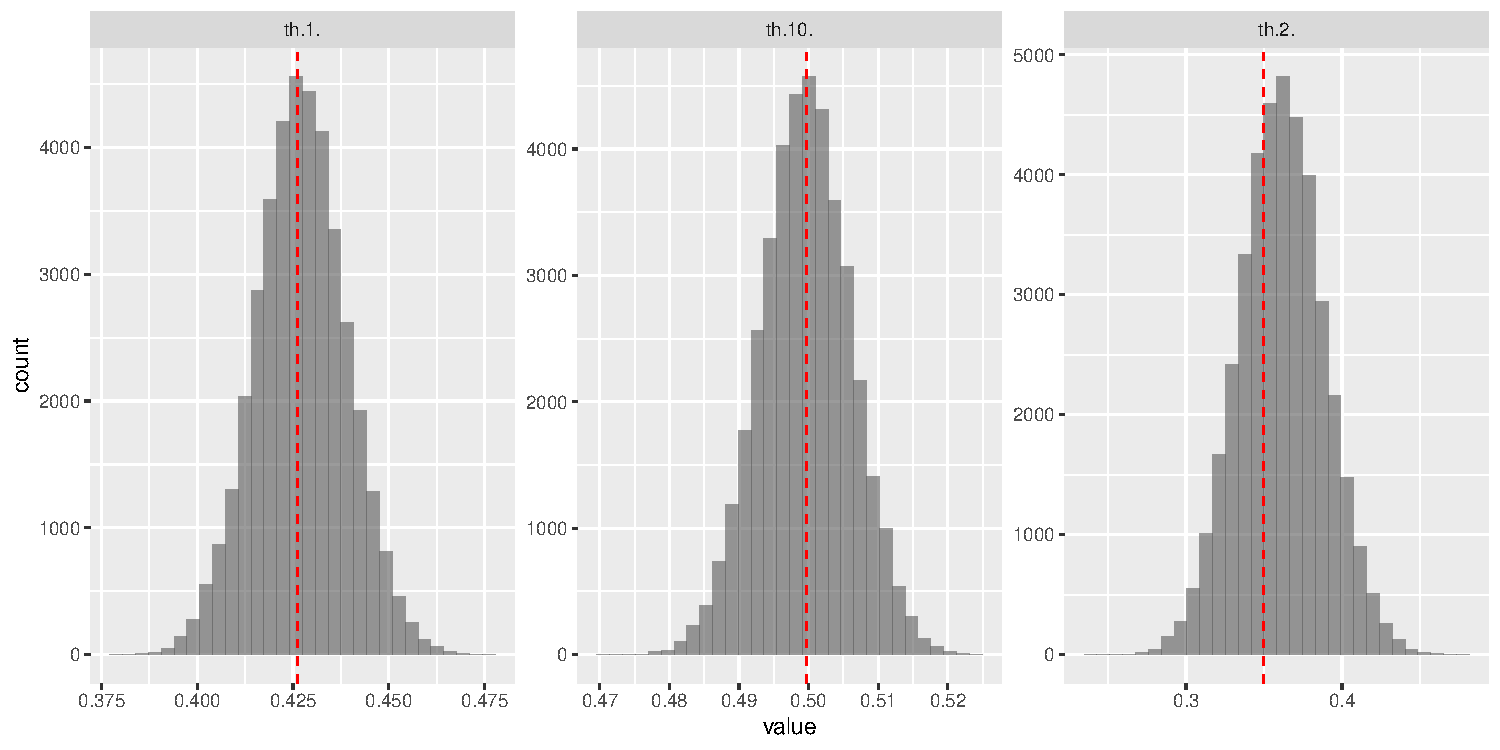
\includegraphics[width=0.9\textwidth]{figs/state_2004_th_hists}
\par\end{centering}
\caption{Simulation results for $\theta_{j}$ (histograms) in comparison with
observed data (red vertical lines). Left, central, and right plots
represent Alabama, Florida, and Alaska respectively. \label{fig:states-binom-sim}}

\end{figure}

In figure \ref{fig:state_time_dep} you can see how electoral mood
of different states changes with time. It is interesting to note that
Alaska (blue line) is becoming more democratic, while Alabama (red
line) tends to be more republican. It does not mean, however, that
they changed their preferences completely: on the whole data range
we see $\theta_{j}<0.5$ for these two states. It is not the fact,
however, for Florida (green line), which crossed middle line $\theta=0.5$
several times during last 20 years.

\begin{figure}
\begin{centering}
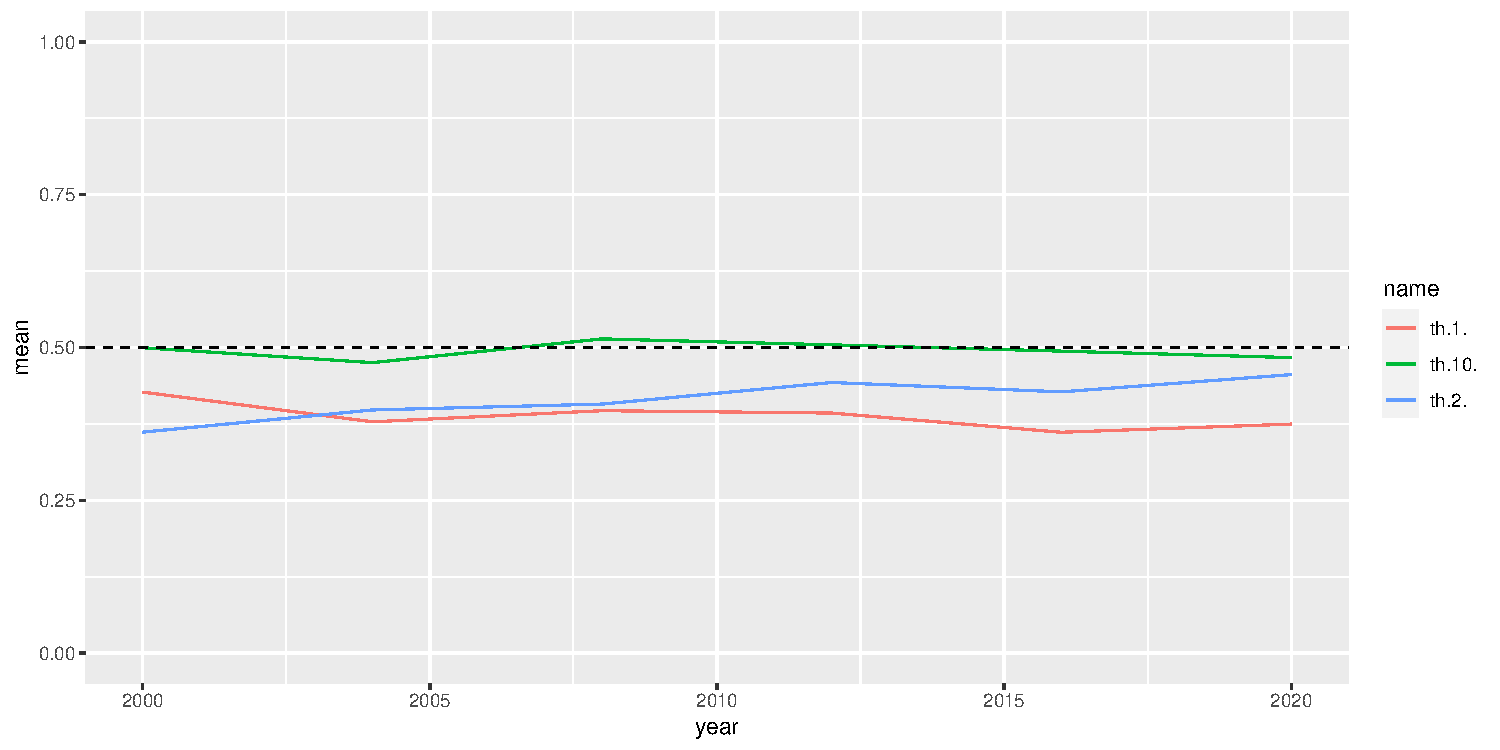
\includegraphics[width=0.9\textwidth]{figs/state_time_dep}
\par\end{centering}
\caption{\label{fig:state_time_dep}}

\end{figure}


\subsection{Normal Model}

\subsubsection{Description}

The alternative way to describe the same dataset is to use normal
distributions. Number of people participating in the elections is
large enough, so this approach can also give good results.

In this model I will talk not about proportions $\theta_{j}$, but
about logits
\begin{align*}
y_{j}= & \log\frac{\theta_{j}}{1-\theta_{j}}=\log\frac{D_{j}}{V_{j}-R_{j}}.
\end{align*}
This change of the variable is typical for categorical variables since,
in contrast to the proportion $\theta_{j}$, the logit is not required
to be in $\left[0;1\right]$ range. Backward transformation from logits
to original proportions is straightforward:
\begin{align*}
\theta_{j}= & \frac{e^{y_{j}}}{1+e^{\theta_{j}}}.
\end{align*}
Since the logit can take any real value, it is fine to model it using
normal sampling distribution
\begin{align*}
y_{j}|\nu_{j}\sim & N\left(\nu_{j},\sigma_{j}^{2}\right),
\end{align*}
where
\begin{align*}
\sigma_{j}^{2}= & \frac{1}{D_{j}}+\frac{1}{V_{j}-D_{j}}
\end{align*}
is associated with the logit variance and mean $\nu_{j}$ is different
for each state. In the Bayesian approach these means are also random
variables following the normal prior distribution
\begin{align*}
\nu_{j}|\mu,\tau^{2}\sim & N\left(\mu,\tau^{2}\right).
\end{align*}
For hyper-parameters $\mu$ and $\tau^{2}$ we can use some non-informative
prior distribution, for example
\begin{align*}
\mu,\tau^{-2}\sim & \text{unif}.
\end{align*}

In figures \ref{fig:states_2004_hyper_norm_scatter}, \ref{fig:state_2004_norm_th_mean_var}
you can see scatter plot of the hyper-parameters and histograms. It
turns out that $\hat{\theta}$ histograms, generated by binomial and
normal models are very close to each other. The same is true also
for distributions over election percentages, so I will not repeat
figure \ref{fig:states-binom-sim} here.

\begin{figure}
\begin{centering}
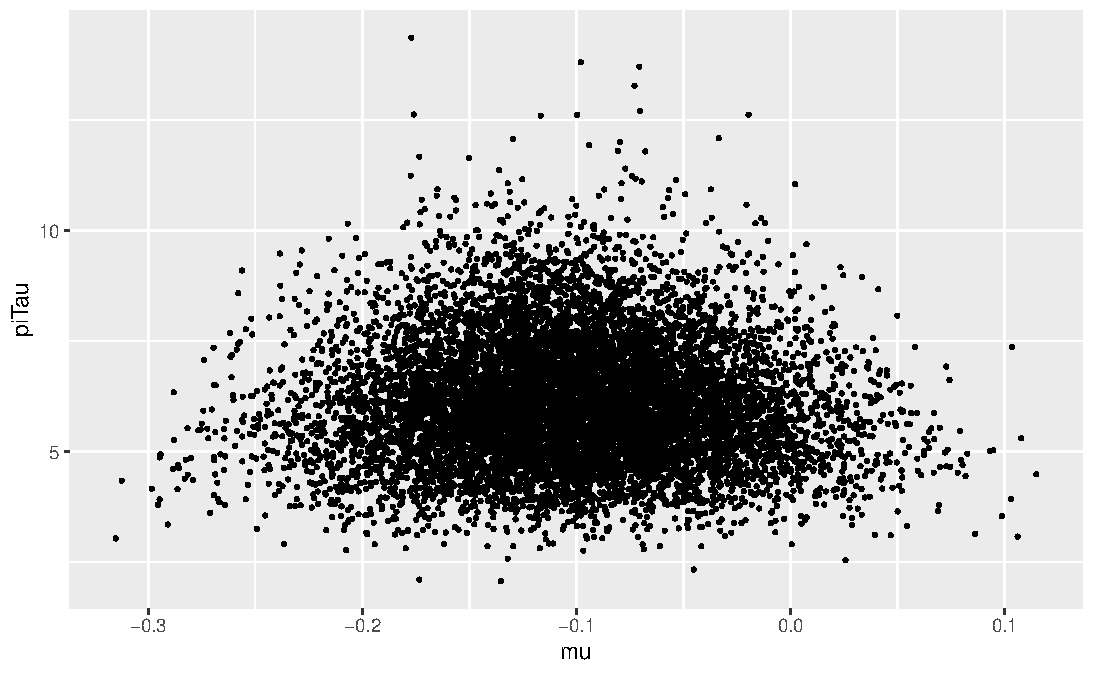
\includegraphics[width=0.9\textwidth]{figs/states_2004_hyper_norm_scatter}
\par\end{centering}
\caption{Scatter Plot of hyper-parameters\label{fig:states_2004_hyper_norm_scatter}}
\end{figure}

\begin{figure}
\begin{centering}
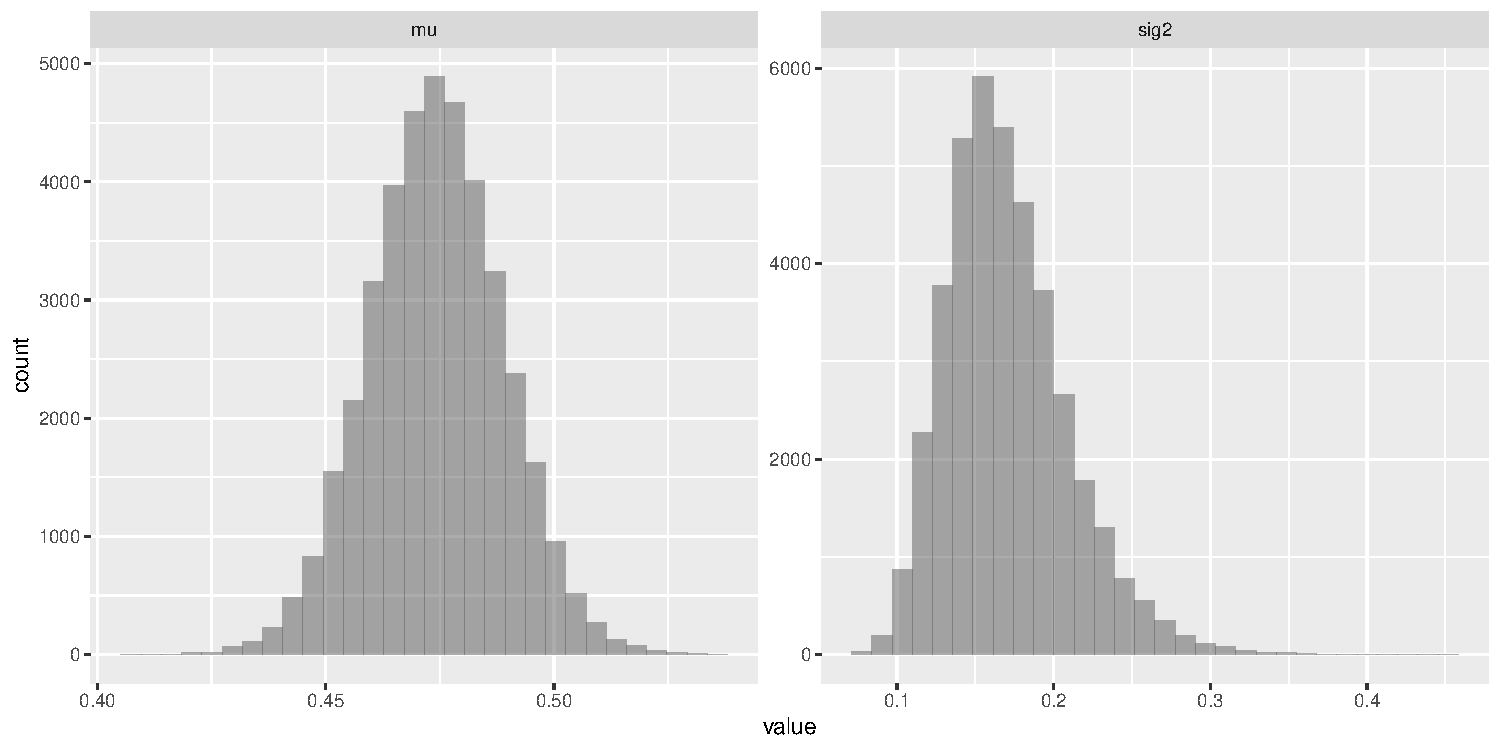
\includegraphics[width=0.9\textwidth]{figs/state_2004_norm_th_mean_var}
\par\end{centering}
\caption{Histograms of $\theta$ mean and variance\label{fig:state_2004_norm_th_mean_var}}
\end{figure}


\subsection{Model Comparison}

As you can see, we have two models that seem to describe equally well
all available data on presidential elections in US on the state level.
The question arises which of them is better for prediction. One of
the ways to answer this question is to use some of Bayesian information
criteria for comparison.

In the following I will discuss Deviance Information criterion (DIC).
In the case of the first (binom) model, for example, this metric is
a difference of two estimates of log-likelyhood functions:
\begin{align*}
p_{DIC}= & 2\left[\log p\left(y|\hat{\theta}_{Bay}\right)-\Epost\log p\left(y|\theta\right)\right],
\end{align*}
where
\begin{align*}
p\left(y|\theta\right)= & \prod_{j}p_{\text{binom}}\left(y_{j}|\theta_{j},V_{j}\right)
\end{align*}
is the posterior probability of the observed data 
\begin{align*}
\hat{\theta}_{Bay}= & \Epost\theta=\frac{1}{S}\sum_{s=1}^{S}\theta^{(s)}.
\end{align*}

Numerical calculations show, that for year 2000 binomial model gives
us
\begin{align*}
\log p\left(y|\hat{\theta}_{Bay}\right)\approx & -368.0,\qquad\Epost\log p\left(y|\theta\right)\approx-394.5,
\end{align*}
which gives us
\begin{align*}
DIC_{\text{binom}}= & -p_{DIC}\approx-51.0.
\end{align*}

In the case of the second (normal) model the expressions are almost
the same. The only difference is that now model parameters are $\nu_{j}$
and the joint posterior probability is equal to
\begin{align*}
p\left(y|\nu\right)= & \prod_{j}p_{\text{norm}}\left(y_{j}|\nu_{j},\sigma_{j}^{2}\right).
\end{align*}
Numerical calculations give us
\begin{align*}
\log p\left(y|\hat{\nu}_{Bay}\right)\approx & 274.2,\qquad\Epost\log p\left(y|\theta\right)\approx248.8,\\
DIC_{norm}\approx & -50.9.
\end{align*}
As we can see, accuracies of two considered models are very close
to each other, but binomial model seems to be slightly better. This
makes sense since binomial distribution is more appropriate for the
considered problem.

\section{County-Level Analysis}

\subsection{Dataset Description}

As we have seen in the previous sections, political preferences of
different states differ significantly. Moreover, while some of the
states are consistently democratic or republican, some others (so
called swing states) change their position pretty often, changing
abruptly the whole picture. It could be very interesting to try to
find some reasons for such differences and changes. A more detailed
analysis, however, show that each state is not uniform, political
preferences of various towns and cities in one state can differ significantly.
This tells us the state is a too large unit and we should consider
smaller units, e.g. counties.

The considered above data set contains information about collected
in 2000-2020 years votes not only on state level, but also for each
county of each state, so we can use this information source for more
detailed analysis. It could be also interesting to use some data about
economic and social situation in counties, that can influence the
political preferences. Such data can be found, for example, on the
official site of the Federal Reserve Bank \citet{FRED}. On this site
for each county you can find detailed information about population,
personal income inequality, etc. You can download tables that you
need both directly from the browser, or using advanced API. The last
method is much more convenient for bulk downloads, so I have used
it.

\subsection{Binomial Model}

Let me first repeat the analysis from previous section on the county
level. Since binomial model has shown to be better choice, I will
use only it.

As previously, votes for the democratic party in each county will
be considered as distributed binomially with parameters $\theta_{j}$,
which by themself have the prior beta distribution with uninformative
uniform distribution for hyper-parameters $a$ and $b$. In figures
\ref{fig:county-hyper-scatter}, \ref{fig:county-hyper-hist} you
can see posterior scatter plot these hyper-parameters and the posterior
mean and variance of the distribution parameter $\theta$. It is clear,
that in comparison with the state level (see figure \ref{fig:state-binom-mean-var}),
mean value of $\theta$ is smaller and the histogram is wider. The
reason for the latter difference is clear: number of votes on county
level are small in comparison with state level, so more variances
are expected.

\begin{figure}
\begin{centering}
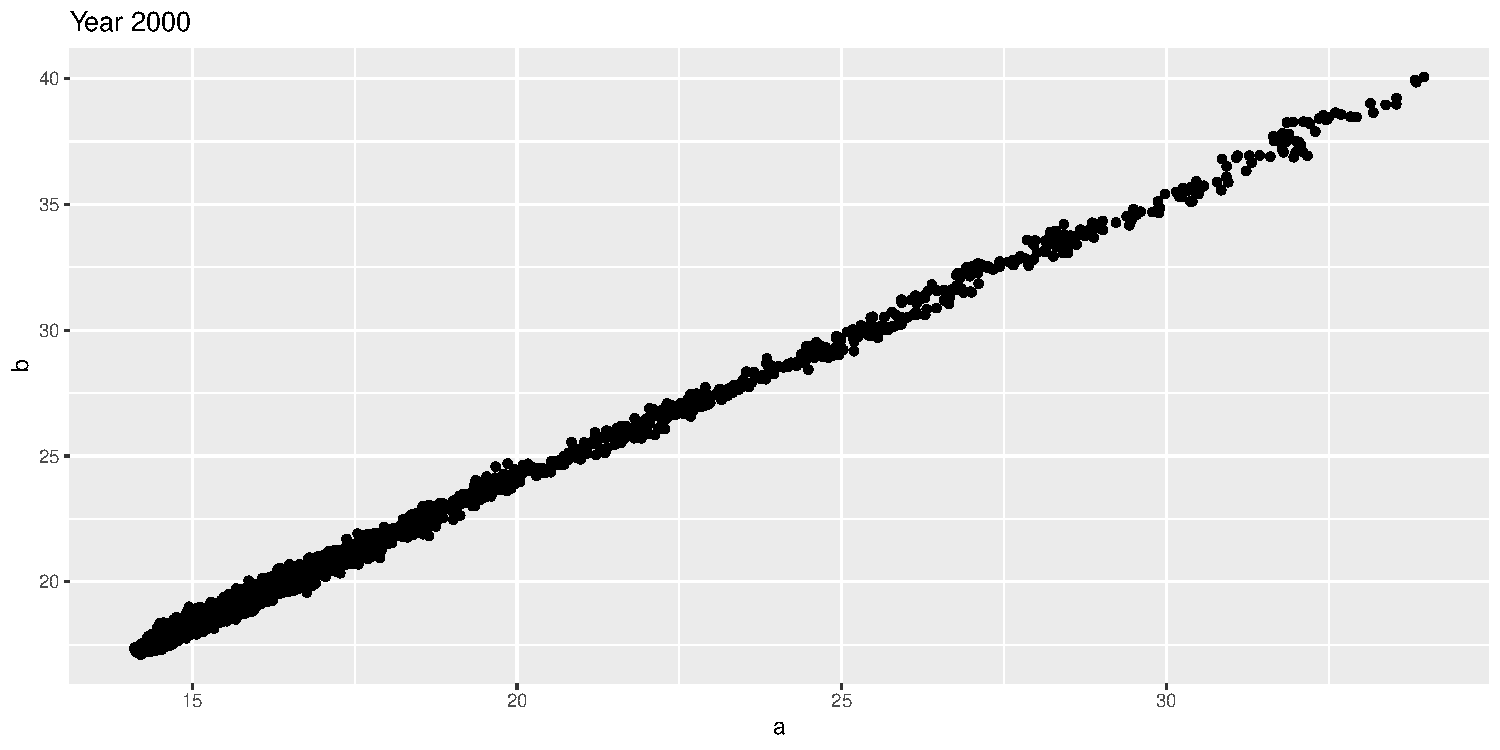
\includegraphics[width=0.9\textwidth]{figs/byCounty/hyperScatter}
\par\end{centering}
\caption{Posterior scatter of the hyper-paarameters on the county level\label{fig:county-hyper-scatter}}

\end{figure}

\begin{figure}
\begin{centering}
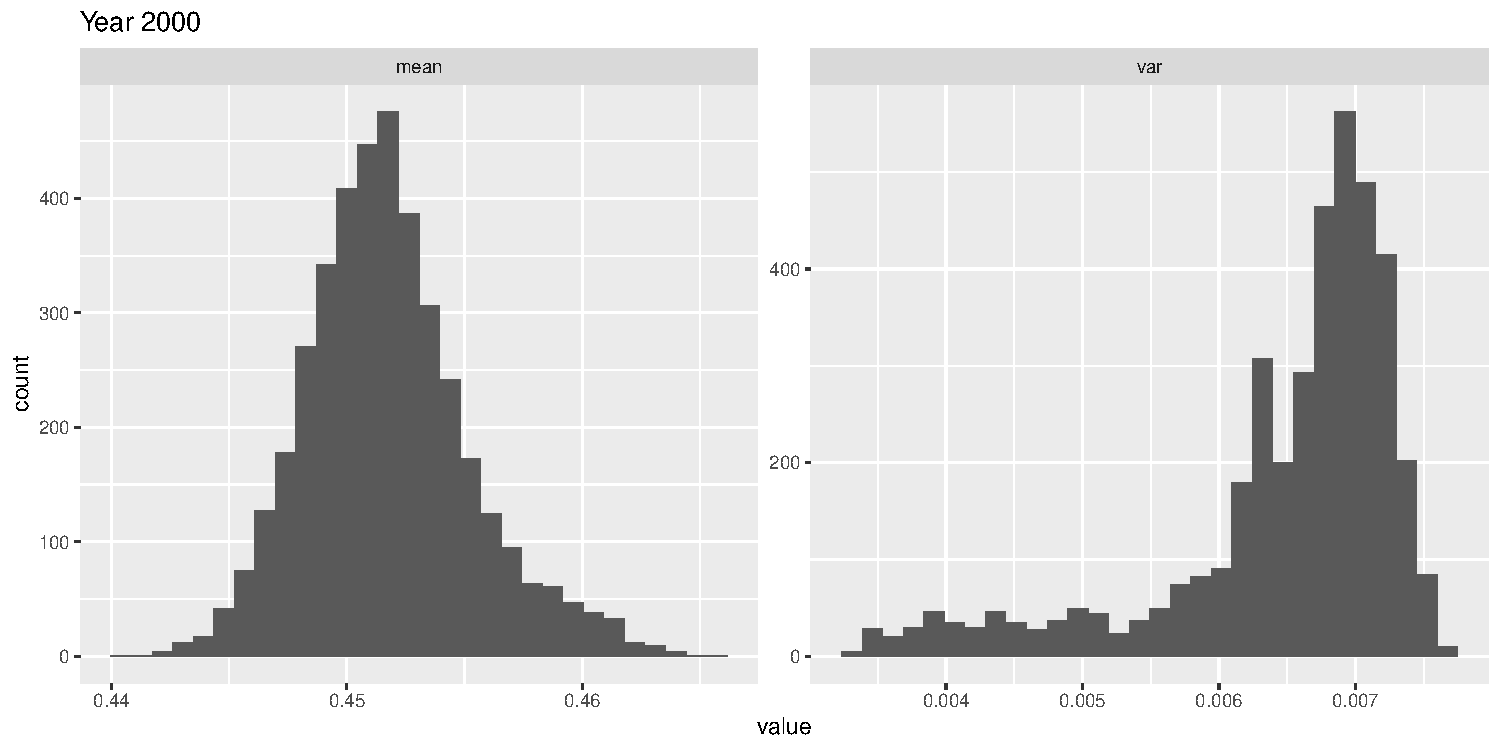
\includegraphics[width=0.9\textwidth]{figs/byCounty/hyper-hist}
\par\end{centering}
\caption{Posterior scatter of the hyper-paarameters on the county level\label{fig:county-hyper-hist}}
\end{figure}

The same result can be clearly seen in figure, where simulation results
for 3 counties are compared with the actual data. As you can see,
peaks of the distributions agree perfectly with the numbers, but the
uncertaintintess are noticeable. 

\begin{figure}
\begin{centering}
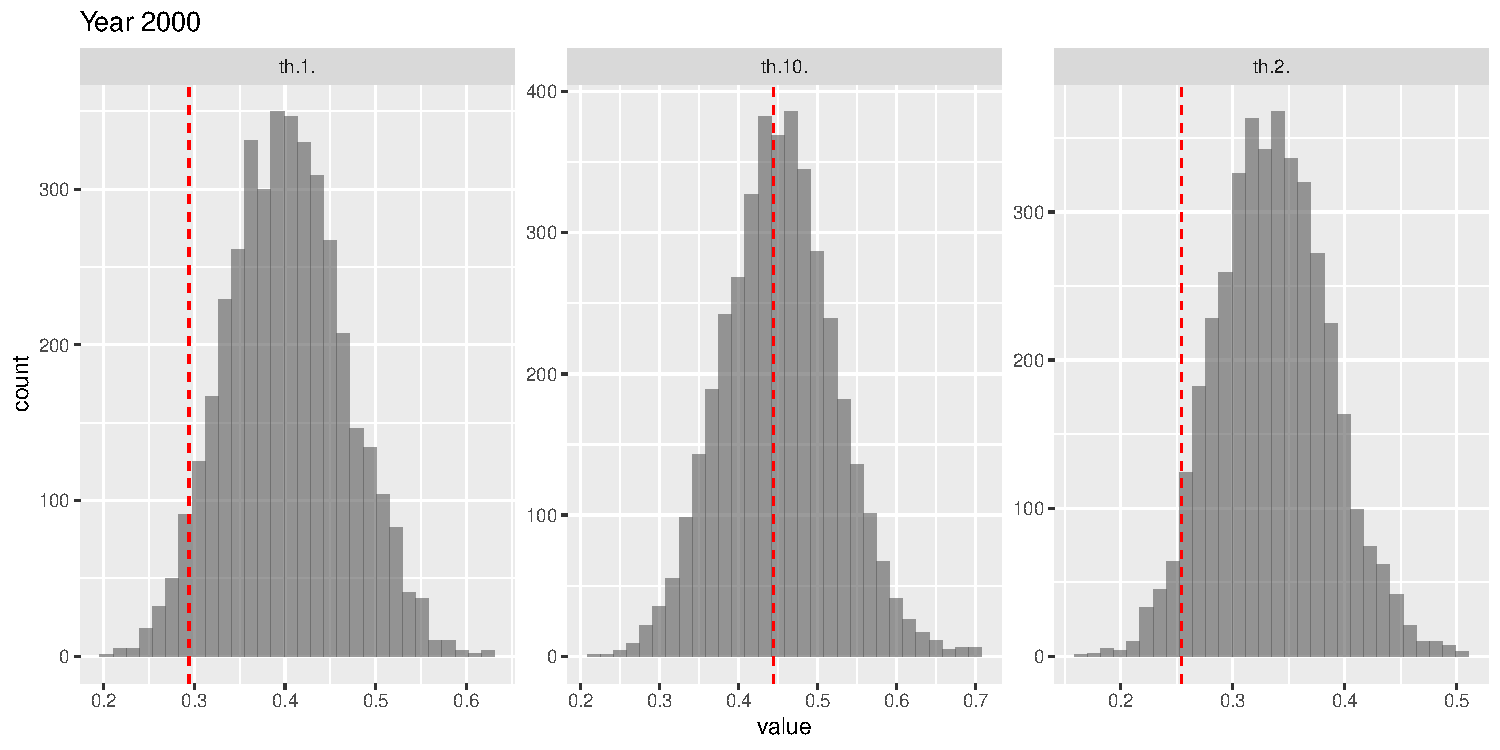
\includegraphics[width=0.9\textwidth]{figs/byCounty/th-hists}
\par\end{centering}
\caption{Posterior scatter of the hyper-paarameters on the county level, Left,
center and right panels correspond to Autauga, Cherokee, and Baldwin
counties (Alabama state) \label{fig:county-th-hist-1}}
\end{figure}

The last interesting figure that I would like to show in this section
is the dependence of the political prefrences on the population of
the county. As you can see from figure \ref{fig:county-th-V}, the
correlation is not very prominent, but we can suggest that with the
increase of the population percentage of votes in favor of democratic
party increases. The effect is better seen on the right panel of the
figure, where logarithmic scale is used for both axis.

\begin{figure}
\begin{centering}
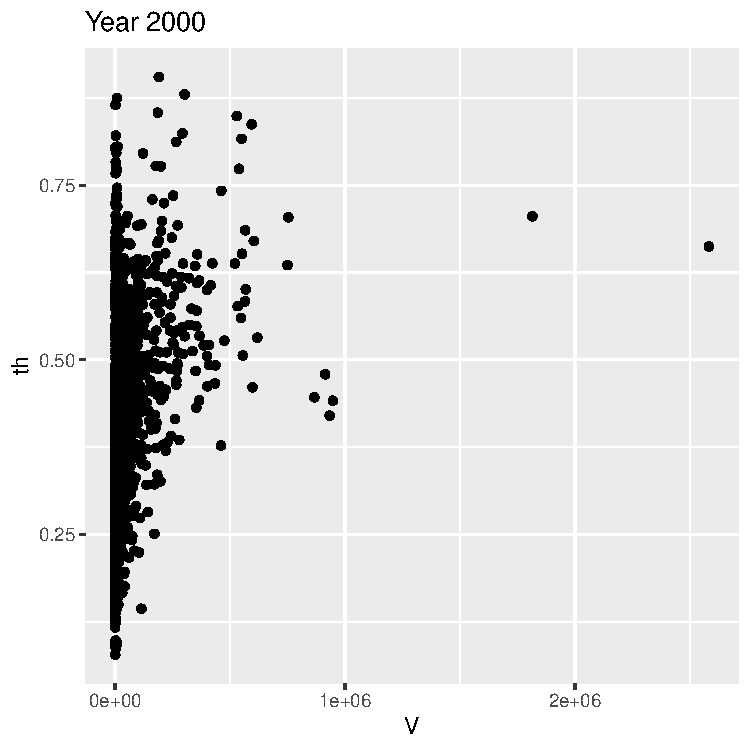
\includegraphics[width=0.45\textwidth]{figs/byCounty/V-th}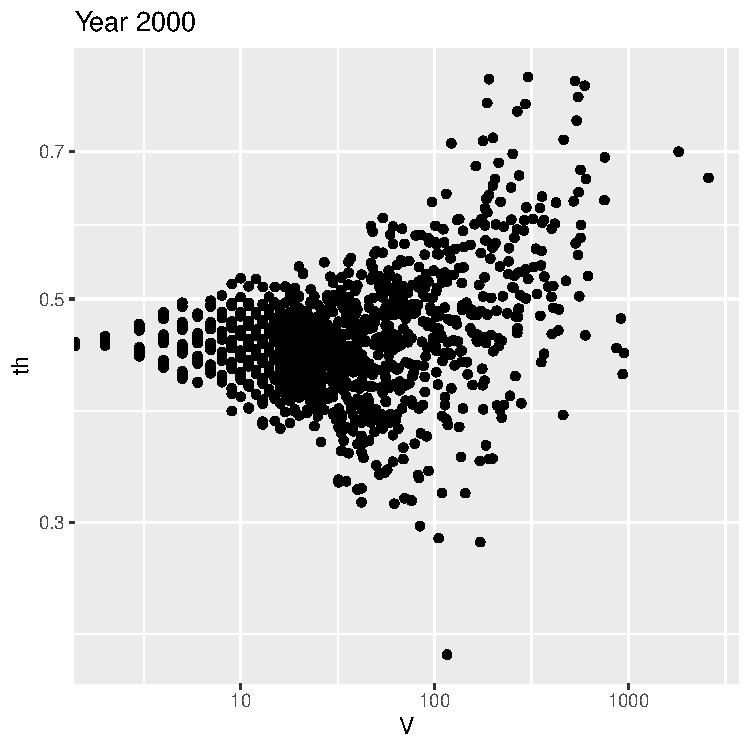
\includegraphics[width=0.42\textwidth]{figs/byCounty/V-th-log}
\par\end{centering}
\caption{Posterior scatter of the hyper-paarameters on the county level, Left,
center and right panels correspond to Autauga, Cherokee, and Baldwin
counties (Alabama state) \label{fig:county-th-V}}
\end{figure}


\subsection{Linear Regression}

This result shows, that there could be some hope to determine the
political preferences of the county using various social and economic
factors as predictors. As it was mentioned earlier, Federal Reserve
Bank database provides us such information for all the counties. In
this subsection I will consider some of them. For simplicity only
situation with the Ohio state counties will be considered in this
subsection and we will restrict ourself to year 2000.

In total there are 87 counties in Ohio and for each of them number
of votes for democratic and republican parties are know. As previously,
in our Bayesian approach we will use binomial sampling distribution
\begin{align*}
D_{i}|\theta_{j}\sim & \text{binom}\left(\theta_{j},V_{j}\right)
\end{align*}
will be used, but now we will determine how distribution parameters
$\theta$ depends on such predictors as
\begin{itemize}
\item total number of votes,
\item Income Inequality, that is the ratio of the mean income for the highest
quintile (top 20 percent) of earners divided by the mean income of
the lowest quintile (bottom 20 percent) of earners in a particular
county,
\item Real Gross Domestic Product, which is is a measure of the market value
of final goods and services produced within a county area in a particular
period,
\item Per Capita Personal Income, that is the income that is received by
persons from all sources.
\end{itemize}
In the following they will be denoted as $V_{j}$, $\mathrm{IR}_{j}$,
$\text{GDP}_{j}$, and $\text{PCI}_{j}$ respectively.

The simplest model to use in this case is Multiple linear model. It
cannot be applied directly to $\theta_{j}$ since allowed value range
for this parameter is $\theta_{j}\in\left[0;1\right]$. As previously,
this problem can be used if we consider not the preference proportions
themselves, but the logits
\begin{align*}
y_{j}= & \log\frac{\theta_{j}}{1-\theta_{j}}=\log\frac{D_{j}}{R_{j}}.
\end{align*}
This means that in this section we are using the model
\begin{align*}
D_{j}|\theta_{j}\sim & \text{binom}\left(\theta_{j},V_{j}\right),
\end{align*}
where the prior distribution for the the logits is
\begin{align*}
y_{j}|a,b_{0},b_{V},b_{\text{IR}},b_{\text{GDP}},b_{\text{PCI}}= & \log\frac{\theta_{j}}{1-\theta_{j}}\sim b_{0}+b_{V}V_{j}+b_{\text{IR}}\text{IR}_{j}+b_{\text{GDP}}\text{GDP}_{j}+b_{\text{PCI}}\text{PCI}_{j}.
\end{align*}
It should be noted that model parameters $b_{0}$, $b_{\text{IR}}$,
$b_{\text{GDP}}$, and $b_{\text{PCI}}$ are universal (i.e. the same
for all counties in the Ohio state). We have selected the simplest
non-informative prior distribution for these parameters:
\begin{align*}
b_{i}\sim & \text{unif}\left(-1000,1000\right),
\end{align*}
where the limiting values were selected to be large enough to capture
all possible range.

Let us first compare model predictions with the observed values, and
then discuss the fitting results. In figure \ref{fig:Ohio_LR_comparison}
you can see results, obtained with the simplest possible model (intercept
only) and some others with increasing complexity. As you can see,
the zero approximation gives us a reasonable result, and even after
addition of the first predictor (inequality ration, $\text{IR}_{j}$)
agreement improves significantly. More complex models also give us
some increase in accuracy.

\begin{figure}
\begin{centering}
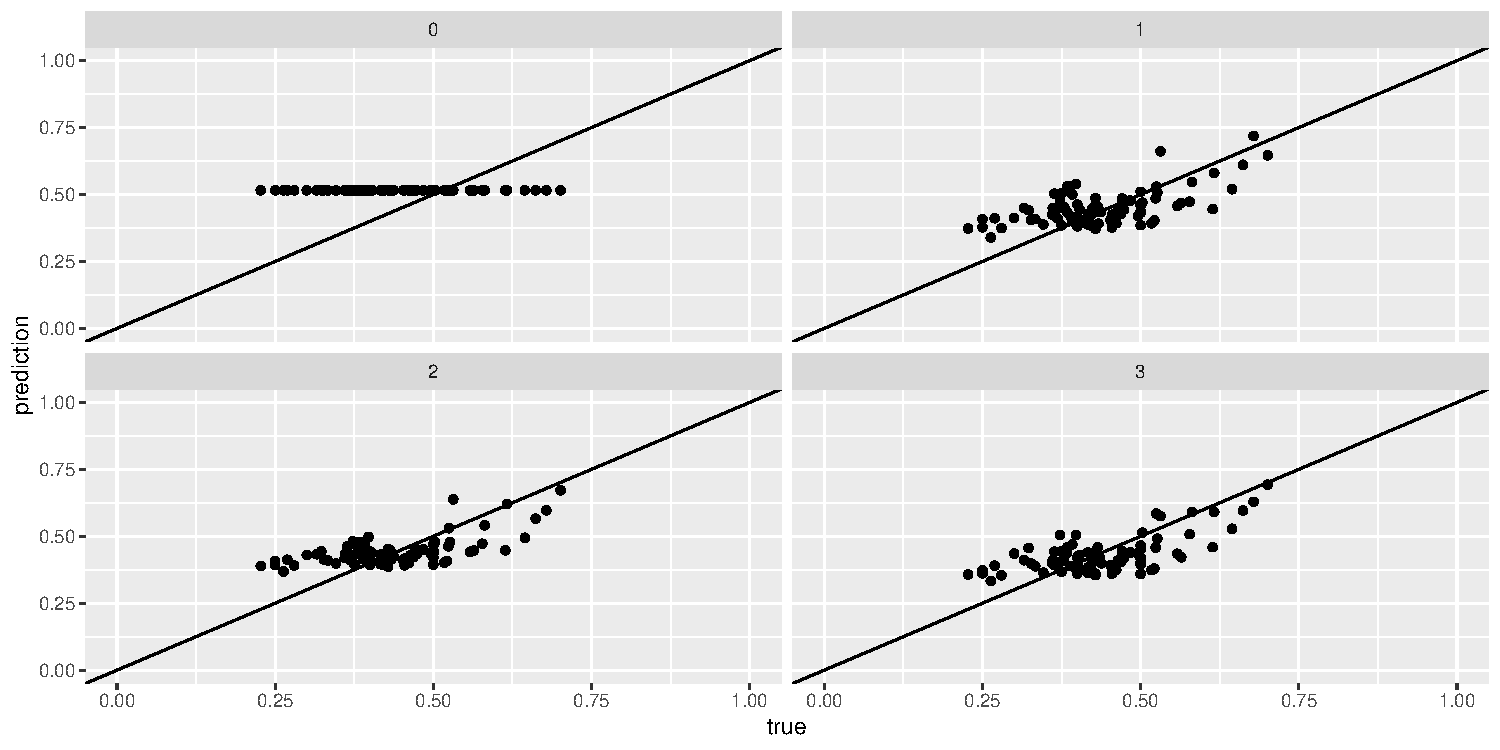
\includegraphics[width=0.9\textwidth]{figs/byCounty/Ohio_LR_comparison}
\par\end{centering}
\caption{Comparison of the linear models' predictions with true values. Labels
0, 1, 2, 3 correspond to models $y=b_{0}$, $y=b_{0}+b_{\text{IR}}\text{IR}$,
$y=b_{0}+b_{\text{IR}}\text{IR}+b_{\text{V}}\text{V}$, and $y=b_{0}+b_{\text{IR}}\text{IR}+b_{\text{V}}\text{V}+b_{\text{GPD}}\text{GPD}$
respectively\label{fig:Ohio_LR_comparison}}
 

\end{figure}

In figure \ref{fig:Ohio_LR_pairs} you can see the posterior scatter
plot of the hyper-parameters. Determined from the simulations posterior
means and standard deviations are
\begin{align*}
\E b_{0}= & -0.8524, & \sqrt{\var b_{0}}= & 0.0086,\\
\E b_{\text{IR}}= & 0.09002, & \sqrt{\var b_{\text{IR}}}= & 0.000558,\\
\E b_{\text{V}}= & 4.285\times10^{-6} & \sqrt{\var b_{\text{V}}}= & 2.50\times10^{-8},\\
\E b_{\text{gpd}}= & -2.517\times10^{-8} & \sqrt{\var b_{\text{gpd}}}= & 1.88\times10^{-10},\\
\E b_{\text{pci}}= & -1.569\times10^{-5} & \sqrt{\var b_{\text{pci}}}= & 1.566\times10^{-7}.
\end{align*}
As you can see, all the predictors seem to be significant. It is interesting
to note, that the coefficient of the $\text{IR}$ predictor is positive,
meaning that high inequality increase the chances of the democratic
party. The coefficients $b_{\text{GPD}}$, $b_{\text{PCI}}$, on the
other hand, are negative. One should keep in mind, however, that according
to figure \ref{fig:Ohio_LR_pairs} these predictors are strongly correlated.

\begin{figure}
\begin{centering}
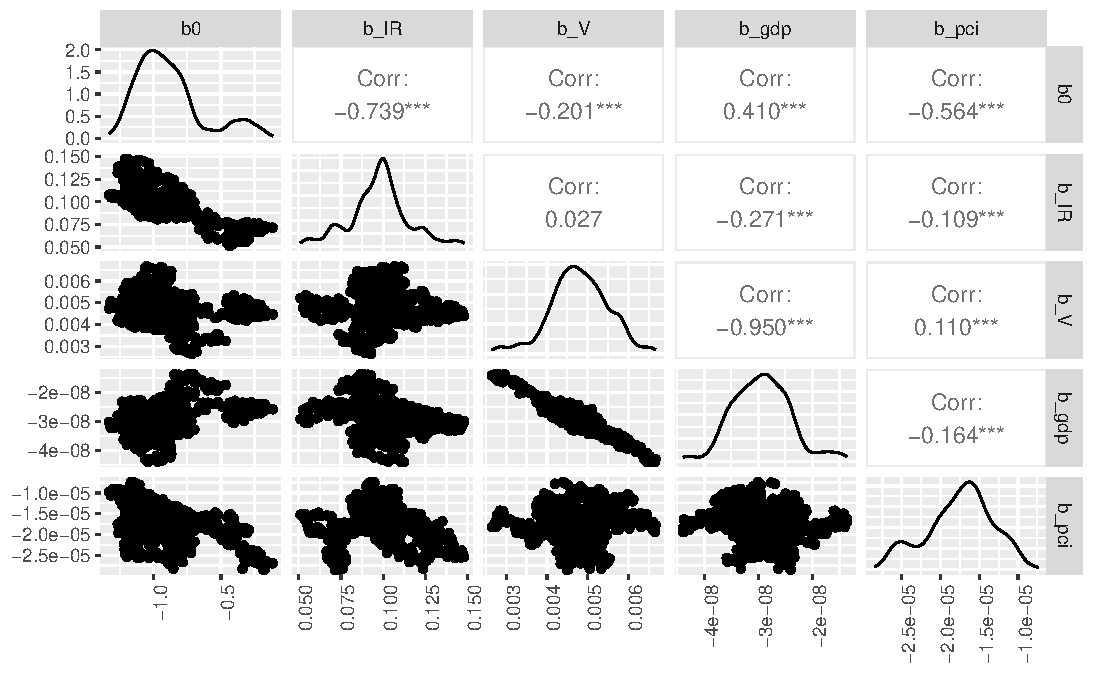
\includegraphics[width=0.9\textwidth]{figs/byCounty/Ohio_LR_pairs}
\par\end{centering}
\caption{Pairs plots for the linear-model hyper-parameters\label{fig:Ohio_LR_pairs}}

\end{figure}


\section{Conclusion}

\bibliographystyle{unsrturl}
\bibliography{math6480_project}


\appendix

\section{Backup}

\subsection{By state, simulation}

With the described above model the posterior distribution of the logits
$\nu_{j}$ has the form
\begin{align*}
\nu_{j}|\mu,\tau^{2},y_{j}\sim & N\left(\hat{\nu}_{j},\hat{\sigma}_{j}^{2}\right),
\end{align*}
where
\begin{align*}
\hat{\nu}_{j}= & \frac{y_{j}\pi_{j}+\mu\pi_{\tau}}{\pi_{j}+\pi_{\tau}},\qquad\hat{\sigma}_{j}^{2}=\frac{1}{\pi_{j}+\pi_{\tau}}
\end{align*}
while $\pi_{j}=\sigma_{j}^{-2}$ and $\pi_{\tau}=\tau^{-2}$ are precisions
of the observed data and hyper-parameters respectively.

Now the simulation process looks like follows:
\begin{enumerate}
\item Draw large number of hyper-parameters $\mu$, $\tau^{2}$ from the
non-informative prior distribution
\item For each state $j$ calculate posterior distribution parameters $\hat{\nu}_{j}$,
$\hat{\sigma}_{j}^{2}$;
\item From the posterior distribution draw means $\nu_{j}$
\item From the sampling distribution draw logits $y_{j}$
\item Calculate the proportions $\theta_{j}$.
\end{enumerate}
In comparison with binomial model this procedure looks more complicated,
but we are not dealing here with any unknown distributions, like the
one presented in relation (\ref{eq:state-binom-hyperpost}).
\end{document}
